\section{LoRA Fine-Tuning Protocol}
\label{app:lora_protocol}

Table~\ref{tab:lora_protocol} lists the full LoRA fine-tuning configuration used for recursive chain construction (\S\ref{sec:method:benchmark}).
At each depth $k$, a fresh LoRA adapter is initialized on the base model and trained on $\mathcal{D}_{k-1}$; adapters are not inherited across depths.
The HuggingFace Trainer default linear decay schedule is used with no warmup.
Target modules are model-specific: \texttt{query\_key\_value} (Pythia), \texttt{att\_proj} (OLMo), and \texttt{c\_attn} (GPT-2~XL).
Cross-scale 7--8B experiments (Appendix~\ref{app:cross_scale_full}) use QLoRA (4-bit NF4) with $r{=}16$, $\alpha{=}32$; the 14B model uses FP16 LoRA with the same rank and scaling.

\begin{table}[h]
\centering
\small
\caption{LoRA fine-tuning hyperparameters for the primary 1--1.5B benchmark. Identical across all three model families and all depth levels.}
\label{tab:lora_protocol}
\begin{tabular}{@{}ll@{}}
\toprule
Parameter & Value \\
\midrule
LoRA rank $r$ & 16 \\
LoRA alpha $\alpha$ & 32 \\
LoRA dropout & 0.05 \\
Bias & none \\
Epochs per depth & 3 \\
Learning rate & $2 \times 10^{-4}$ \\
LR schedule & linear decay (no warmup) \\
Batch size (effective) & 16 ($8 \times 2$ grad.\ accum.) \\
Max sequence length & 512 tokens \\
Precision & bfloat16 \\
Adapter init & from scratch (base model) \\
Seed & 42 (primary), 43 (replication) \\
\bottomrule
\end{tabular}
\end{table}

\section{Additional Results}
\label{app:additional}

\subsection{Top-$k$ Feature Trajectories}
\label{app:topk_trajectories}

Feature trajectories for nucleus and temperature sampling appear in Figure~\ref{fig:feature_trajectory} (\S\ref{sec:atlas:edd}).
Top-$k$ ($k{=}50$) trajectories follow the same monotonically decreasing trend for all features but with compressed inter-depth spacing, consistent with the signal attenuation effect discussed in \S\ref{sec:atlas:strategy}.
Concretely, the d0$\to$d1 drop in \texttt{p90\_ppl} under top-$k$ is 78\% (vs.\ 87\% for nucleus), and the d2$\to$d3 reduction is 31\% (vs.\ 39\% for nucleus).
Despite the magnitude reduction, feature rank ordering across depths is preserved, which explains why ordinal classifiers maintain directionality even under top-$k$ conditions.

\subsection{Permutation Importance}
\label{app:permutation}

To verify that the Gini-based importance rankings in \S\ref{sec:atlas:features} are not an artifact of the impurity measure, we compute permutation importance (5-fold CV, 10 repeats) for all 9 atlas cells.
The top-2 features are stable across measures: \texttt{p90\_ppl} ranks in the top 2 in 9/9 cells under both Gini and permutation importance, and \texttt{var\_surprisal} in 8/9 (vs.\ 7/9 for Gini, with the additional cell being OLMo top-$k$; the single SHAP exception is GPT-2~XL top-$k$, where \texttt{p75\_ppl} displaces \texttt{var\_surprisal} to rank 3).
Kendall's $W{=}0.90$ across all three methods (Gini, permutation, SHAP) indicates strong concordance ($p{<}0.005$).
Pairwise Spearman correlations are: SHAP--Gini $\rho{=}0.93$, SHAP--permutation $\rho{=}0.84$, Gini--permutation $\rho{=}0.76$.
Per-cell top-5 overlap between SHAP and permutation importance is 3--4 out of 5 features; the aggregated (mean-across-cells) top-5 sets are identical; the top features are therefore robust to the choice of importance measure at the aggregate level, though per-cell rankings exhibit model-dependent variation.

\subsection{Conditional Permutation Importance under Multicollinearity}
\label{app:conditional_pi}

With 14--16 of 19 features exhibiting VIF${>}$10 (\S\ref{sec:atlas:features}), standard permutation importance may inflate contributions of correlated features: permuting one member of a collinear set allows others to compensate, masking true individual effects.
We compute conditional permutation importance (CPI) \citep{strobl2008_conditional}, which permutes each feature \emph{within strata defined by its correlated partners}, isolating the unique contribution after controlling for multicollinearity.

\paragraph{Setup.}
CPI is computed on all 9 model$\times$strategy cells.
For each cell, 1{,}000 bootstrap resamples produce a rank distribution per feature; the 95\% bootstrap CI width quantifies rank stability (width $\leq 1.0$ indicates near-invariant rankings across resamples).

\paragraph{Results.}
Table~\ref{tab:conditional_pi} summarizes the top-5 features by mean CPI across cells.
\texttt{var\_surprisal} (avg rank 1.4, CPI\,=\,0.260) and \texttt{p90\_ppl} (avg rank 1.7, CPI\,=\,0.238) are the top-2 in 8/9 cells, with bootstrap rank CI widths of 0.44 and 0.22---both $\leq 0.5$, indicating near-invariant rankings across resamples.
Ranks 3--5 are \texttt{p75\_ppl} (CPI\,=\,0.063, CI width\,=\,0.78), \texttt{p50\_ppl} (0.016, width\,=\,2.67), and a cell-dependent set (\texttt{p25\_ppl} or \texttt{mean\_ppl}); rank stability decreases beyond the top-2, with CI widths of 2.7--3.7 for ranks 4--5.

\begin{table}[h]
\centering
\small
\caption{Conditional permutation importance aggregated across 9 model$\times$strategy cells (1{,}000 bootstrap resamples). Avg Rank and Avg CPI: means over cells. Rank CI Width: mean 95\% bootstrap CI width for the rank. Bottom rows: feature-family averages.}
\label{tab:conditional_pi}
\resizebox{\columnwidth}{!}{%
\begin{tabular}{@{}lccc@{}}
\toprule
Feature / Family & Avg Rank & Avg CPI & Rank CI Width \\
\midrule
\texttt{var\_surprisal} & 1.4 & 0.260 & 0.44 \\
\texttt{p90\_ppl} & 1.7 & 0.238 & 0.22 \\
\texttt{p75\_ppl} & 3.1 & 0.063 & 0.78 \\
\texttt{p50\_ppl} & 5.0 & 0.016 & 2.67 \\
\texttt{p25\_ppl}$^\dagger$ & 5.8 & 0.012 & 3.67 \\
\texttt{mean\_ppl}$^\dagger$ & 6.3 & 0.008 & 3.44 \\
\midrule
Surprisal family & 7.3 & 0.089 & --- \\
Perplexity family & 7.5 & 0.039 & --- \\
Lexical family & 9.7 & 0.004 & --- \\
\bottomrule
\multicolumn{4}{@{}l}{\footnotesize $^\dagger$Rank 5--6 varies by cell; \texttt{trigram\_entropy} appears in 1 cell.}
\end{tabular}}
\end{table}

Two exceptions exist among GPT-2~XL cells: in temperature sampling, \texttt{p90\_ppl} (CPI\,=\,0.419) exceeds \texttt{var\_surprisal} (0.093) while both remain in the top-2; in top-$k$ sampling, \texttt{p90\_ppl} (0.475) and \texttt{p75\_ppl} (0.127) push \texttt{var\_surprisal} to rank~3 (0.037), the only cell where it exits the top-2.
Both reversals are consistent with the Gini rankings for these cells (Table~\ref{tab:feature_importance}).

At the family level, surprisal (avg CPI\,=\,0.089, rank\,=\,7.3) and perplexity (0.039, rank\,=\,7.5) are closely matched, while lexical features (0.004, rank\,=\,9.7) contribute minimally---consistent with the group ablation in \S\ref{sec:atlas:features}.

\paragraph{Consistency with Gini rankings.}
CPI and Gini rankings agree on the dominant feature (\texttt{var\_surprisal} or \texttt{p90\_ppl}) in 8/9 cells; the sole disagreement (GPT-2~XL top-$k$) involves a swap between rank-2 and rank-3 features.
Bootstrap rank CI widths $\leq 0.5$ for the top-2 features confirm that these rankings are not artifacts of collinearity or resampling variability.
Controlling for multicollinearity via conditional permutation corroborates the Gini- and SHAP-based importance hierarchy reported in the main text.

\subsection{Per-Class Recall}
\label{app:per_class}

Table~\ref{tab:per_class_recall} reports per-class recall across all 9 atlas cells (4-class in-distribution, 5-fold CV).
Depth~0 recall exceeds 97\% uniformly.
Among generated depths, d2 is the hardest class in every cell; the deficit is most pronounced under top-$k$ sampling (46--53\%), where vocabulary truncation removes the tail tokens that carry depth-discriminative signal.

\begin{table}[h]
\centering
\small
\caption{Per-class recall (\%) for all 9 atlas cells. d2 is the lowest-recall class in every cell. Boldface marks the highest d2 recall.}
\label{tab:per_class_recall}
\begin{tabular}{@{}lcccc@{}}
\toprule
Cell & d0 & d1 & d2 & d3 \\
\midrule
Pythia, nuc.       & 99.3 & 81.9 & 59.2 & 74.4 \\
Pythia, $\tau$     & 99.2 & 79.9 & 56.0 & 72.1 \\
Pythia, top-$k$    & 98.7 & 71.6 & 44.2 & 60.9 \\
OLMo, nuc.         & 97.8 & 82.1 & 60.6 & 75.3 \\
OLMo, $\tau$       & 99.3 & 87.1 & 65.6 & 77.1 \\
OLMo, top-$k$      & 99.2 & 80.9 & 50.4 & 67.2 \\
GPT-2~XL, nuc.     & 98.5 & 87.4 & 72.8 & 78.5 \\
GPT-2~XL, $\tau$   & 99.0 & 91.1 & \textbf{73.0} & 80.5 \\
GPT-2~XL, top-$k$  & 98.7 & 81.3 & 54.8 & 68.4 \\
\bottomrule
\end{tabular}
\end{table}

\subsection{Confusion Matrices}
\label{app:confusion_matrices}

\begin{figure}[h]
\centering
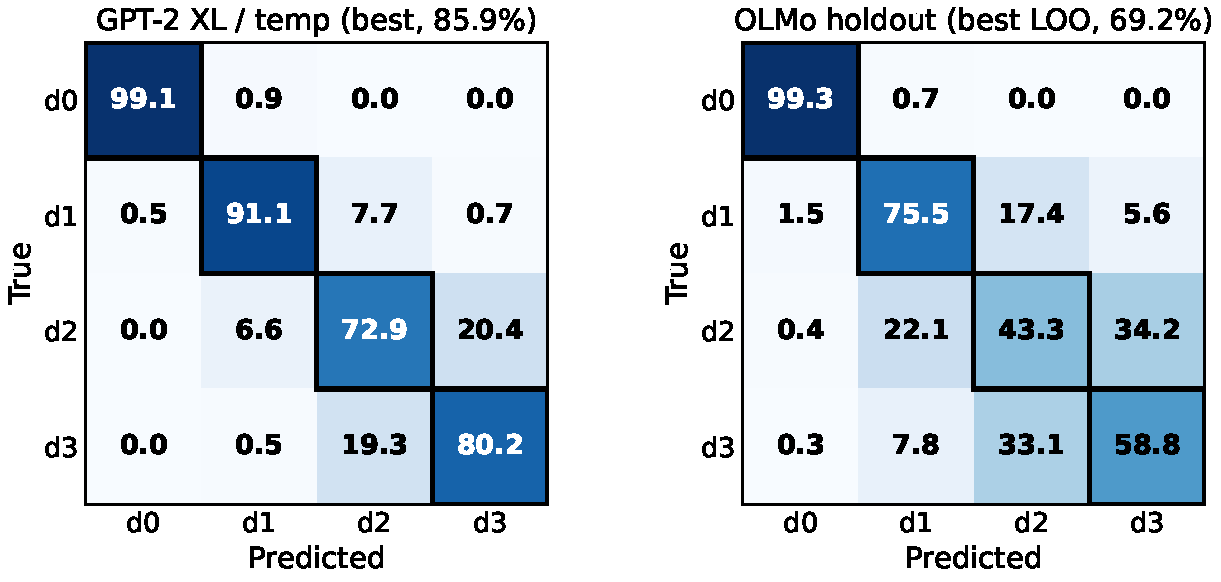
\includegraphics[width=\columnwidth]{figures/fig_confusion_matrix.pdf}
\caption{Confusion matrices: best in-distribution (GPT-2 XL temp, 85.9\%) and best LOO transfer (OLMo, 69.2\%). d0 recall ${>}$99\%; errors spread to d1--d3 under transfer.}
\label{fig:confusion_matrix}
\end{figure}

\subsection{Cross-Strategy Transfer Details}
\label{app:cross_strategy}

\begin{table}[h]
\centering
\small
\caption{Cross-strategy transfer (leave-one-out). Chance = 25\% / 33\% (d1--d3). d0 recall $\geq$89\% inflates headline; d1--d3 mean: 45.9\%.}
\label{tab:cross_strategy}
\begin{tabular}{lccc}
\toprule
Holdout & Pythia & OLMo & GPT-2 XL \\
 & Acc (\%) & Acc (\%) & Acc (\%) \\
\midrule
nucleus & \textbf{69.4} & \textbf{65.4} & \textbf{59.9} \\
temp ($\tau{=}0.9$) & 62.8 & 58.2 & 56.1 \\
top-$k$ ($k{=}50$) & 51.5 & 54.9 & 53.6 \\
\bottomrule
\end{tabular}
\end{table}

\subsection{Accumulation Pairwise AUC}
\label{app:accumulation_auc}

Table~\ref{tab:accum_auc} reports pairwise AUC for the six accumulation cells (3 models $\times$ 2 mixing ratios; GPT-2~XL and Pythia use nucleus, OLMo uses temperature 0.9).
At 25\% mixing, all three cells preserve $\mathrm{EDD}_{0.70}{=}3$.
At 50\% mixing, GPT-2~XL nucleus is the sole failure: d2v3 AUC\,=\,0.695, marginally below the 0.70 threshold (0.55\,pp).

\begin{table}[h]
\centering
\small
\caption{Pairwise AUC under accumulation (GPT-2~XL/Pythia: nucleus; OLMo: temp 0.9; binary RF, 5-fold CV). Bold: $\mathrm{EDD}_{0.70}$ boundary failure.}
\label{tab:accum_auc}
\begin{tabular}{@{}llccc@{}}
\toprule
Model & Mix & d0v1 & d1v2 & d2v3 \\
\midrule
GPT-2~XL & 25\% & 1.000 & 0.817 & 0.726 \\
 & 50\% & 1.000 & 0.831 & \textbf{0.695} \\
Pythia & 25\% & 1.000 & 0.809 & 0.749 \\
 & 50\% & 1.000 & 0.793 & 0.716 \\
OLMo & 25\% & 1.000 & 0.848 & 0.759 \\
 & 50\% & 1.000 & 0.817 & 0.726 \\
\bottomrule
\end{tabular}
\end{table}

\subsection{DCOL Iteration Details}
\label{app:dcol_iterations}

Table~\ref{tab:dcol_iterations} summarizes all six DCOL iterations.
DeBERTa-v3-large exhibited systematic numerical instability across five configurations; RoBERTa-large resolved stability but could not close the accuracy gap with feature-based methods.

\begin{table}[h]
\centering
\small
\caption{DCOL iteration summary. All experiments use Pythia-1.4B nucleus data. RF baseline: 78.7\%.}
\label{tab:dcol_iterations}
\resizebox{\columnwidth}{!}{%
\begin{tabular}{@{}llp{2.2cm}p{2.8cm}@{}}
\toprule
Ver. & Backbone & Config & Outcome \\
\midrule
v1 & DeBERTa & FT, m\_lr $10^{-3}$ & Embed.\ collapse (31.5\%) \\
v2 & DeBERTa & FT, m\_lr $10^{-4}$ & OOM \\
v3 & DeBERTa & FT, m\_lr $10^{-4}$ & Forgetting + OOM \\
v4 & DeBERTa & LoRA, m\_lr $10^{-3}$ & Embed.\ collapse \\
v5 & DeBERTa & LoRA, m\_lr $10^{-4}$ & NaN gradients \\
v6 & RoBERTa & FT, grad clip 1.0 & Stable; 64.5\% ($-$13.7pp) \\
\bottomrule
\end{tabular}}
\end{table}

\subsection{Zero-Shot LLM Prompt Template}
\label{app:zeroshot_prompt}

Both DeepSeek V3.2 and Qwen2.5-7B-Instruct use identical prompting.
The system message defines recursive generation depth with per-depth descriptions (depth~0: human-written; depth~1--3: successive LLM generation cycles) and lists expected textual patterns at each depth (vocabulary richness, repetition, coherence).
The user message presents the passage (truncated to ${\approx}$384 words) and requests a JSON response containing an integer depth prediction (0--3), a confidence score, and a one-sentence reasoning.
No in-context examples are provided.

\begin{quote}
\small
\textbf{System:} ``You are an expert at detecting AI-generated text and estimating its generation depth. `Recursive generation depth' refers to how many times a text has been through an LLM generation cycle: Depth~0: Original human-written text [\ldots] Depth~3: Text generated by an LLM given depth-2 text as input. Key patterns by depth: Depth~0 (human): Rich vocabulary [\ldots] Depth~3 (third-gen): Noticeable repetition, formulaic structure [\ldots]''

\textbf{User:} ``Analyze the following text and estimate its recursive generation depth (0, 1, 2, or 3). TEXT: \{text\}. Respond with ONLY a JSON object: \{\texttt{"depth"}: $\langle$int 0--3$\rangle$, \texttt{"confidence"}: $\langle$float 0--1$\rangle$, \texttt{"reasoning"}: $\langle$str$\rangle$\}''
\end{quote}

\subsection{Temperature Robustness}
\label{app:multi_tau}

The cross-strategy results in \S\ref{sec:gen:crossstrategy} use a single temperature ($\tau{=}0.9$).
To test whether depth signal generalizes across temperatures, we repeat the classification pipeline at $\tau \in \{0.5, 0.7, 0.9, 1.1\}$ on Pythia-1.4B.

\paragraph{Within-$\tau$ robustness.}
For $\tau \in [0.5, 0.9]$, d1-vs-d2 AUC exceeds 0.80 (peak 0.851 at $\tau{=}0.7$, comparable to nucleus $p{=}0.95$'s 0.861) and 4-class accuracy ranges from 75.4\% to 77.3\% (Table~\ref{tab:multi_tau_within}); the depth signal is therefore not an artifact of a single temperature.
The same top-5 features (\texttt{var\_surprisal}, \texttt{p90\_ppl}, \texttt{mean\_ppl}, \texttt{mean\_surprisal}, \texttt{p75\_ppl}) dominate across all $\tau$ values with only minor rank-order variation.

\paragraph{Collapse at $\tau{=}1.1$: memorization as prerequisite.}
At $\tau{=}1.1$, 4-class accuracy drops to 57.2\% and d1v2 AUC falls to 0.528.
Training loss reveals the mechanism: at low temperature ($\tau{=}0.5$), fine-tuning loss decreases steeply across recursive depths ($2.27 \to 0.42 \to 0.16$), a sign of rapid memorization of the model's own output.
At $\tau{=}1.1$, loss remains nearly flat ($2.27 \to 1.91 \to 1.85$); high-entropy output resists memorization, so depth-dependent distributional shifts do not accumulate.
This establishes \emph{memorization as a prerequisite} for detectable depth signal: recursive depth is discriminable only when successive fine-tuning iterations progressively reshape the output distribution.

\paragraph{Cross-$\tau$ non-transferability.}
Leave-one-$\tau$-out transfer yields mean accuracy of 46.7\% with mean d1v2 AUC of 0.319 (Table~\ref{tab:multi_tau_cross}), worse than cross-strategy transfer (59.1\%; \S\ref{sec:gen:crossstrategy}).
Holdout $\tau{=}0.5$ produces inverted d1v2 AUC (0.176); different temperatures therefore produce surprisal distributions with incompatible shapes.
This extends the strategy-specificity finding: even within a single decoding family, the feature space is temperature-specific; strategy-conditioned classifiers are therefore necessary.

\paragraph{Ecological validity.}
On WikiText-103 (546 editorial passages), all three model-specific RF classifiers achieve $\geq$98.5\% d0 accuracy despite $+$621\% domain shift in mean perplexity, partly an easy case, as WikiText's higher perplexity places it farther from d1--d3 in feature space.
On noisier web-crawl data (5{,}000 C4 passages), FPR ranges from 4.7\% (OLMo) to 22.4\% (GPT-2~XL), concentrated in template/SEO content with high n-gram repetition (Table~\ref{tab:calibration}); deployment on heterogeneous web data requires model-specific calibration.

\begin{table}[h]
\centering
\small
\caption{Within-$\tau$ 4-class classification (Pythia-1.4B, 5-fold CV, independent pipeline run). d$i$v$j$: pairwise AUC for depth $i$ vs.\ depth $j$. The $\tau{=}0.9$ accuracy (75.9\%) differs from the main atlas (76.8\%, Table~\ref{tab:main_matrix}) due to separate generation and LoRA training runs.}
\label{tab:multi_tau_within}
\resizebox{\columnwidth}{!}{%
\begin{tabular}{@{}lcccc@{}}
\toprule
$\tau$ & 4-class acc (\%) & d1v2 AUC & d0v1 AUC & d2v3 AUC \\
\midrule
0.5 & 77.3 & 0.842 & 0.996 & 0.764 \\
0.7 & 75.4 & 0.851 & 0.997 & 0.720 \\
0.9 & 75.9 & 0.808 & 0.991 & 0.781 \\
1.1 & 57.2 & 0.528 & 0.988 & 0.599 \\
\bottomrule
\end{tabular}}
\end{table}

\begin{table}[h]
\centering
\small
\caption{Cross-$\tau$ leave-one-out transfer (Pythia-1.4B). Train on three temperatures, test on the held-out one.}
\label{tab:multi_tau_cross}
\begin{tabular}{@{}lcc@{}}
\toprule
Holdout & Acc (\%) & d1v2 AUC \\
\midrule
$\tau{=}0.5$ & 52.2 & 0.176 \\
$\tau{=}0.7$ & 41.0 & 0.299 \\
$\tau{=}0.9$ & 46.4 & 0.277 \\
$\tau{=}1.1$ & 47.1 & 0.525 \\
\midrule
Mean & 46.7 & 0.319 \\
\bottomrule
\end{tabular}
\end{table}

\subsection{Feature Overlap Analysis}
\label{app:feature_overlap}

We probe whether end-to-end PLM representations capture the same depth signals as our statistical features via linear probing of [CLS] representations from DeBERTa-v3-base and RoBERTa-base.
PLM representations excel at surface lexical features (TTR: $R^2{=}0.85$, repeated bigrams) but fail to capture perplexity distribution statistics; \texttt{var\_surprisal} and \texttt{p90\_ppl} yield negative $R^2$ under linear probing; these features are not linearly accessible in the pretrained representation space.
This confirms that the 20pp accuracy gap between feature-based and end-to-end methods (\S\ref{app:e2e}) stems from complementary, not redundant, representations: PLMs capture lexical patterns while the targeted statistical features capture distributional tail properties that constitute the dominant depth markers.

\subsection{End-to-End Learning}
\label{app:e2e}

DeBERTa-v3-base \cite{he2021_deberta_v3} and RoBERTa-base \cite{liu2019_roberta} finetuned end-to-end achieve 58.3\% ($\pm$4.7\%) and 59.5\% ($\pm$3.2\%) respectively, lagging the RF baseline (78.7\%) by 20.4pp and 19.2pp.
The 1.2pp inter-backbone gap rules out architecture bias; Table~\ref{tab:e2e_detail} shows both backbones share the same failure mode (high d0 F1, $>$0.94, but collapsed d1/d2 performance, F1 $\leq$ 0.42), while RF achieves 0.596 d2 recall, a $>$2$\times$ advantage at the hardest depth class.

\begin{table}[h]
\centering
\small
\caption{Per-class performance for end-to-end PLM classifiers vs.\ RF baseline (Pythia-1.4B nucleus). PLM columns report F1; RF d2 column reports recall (the class with the largest PLM--RF gap). Both PLM backbones share the same failure pattern: collapsed d1/d2 scores despite adequate d0/d3.}
\label{tab:e2e_detail}
\resizebox{\columnwidth}{!}{%
\begin{tabular}{@{}lccccc@{}}
\toprule
Method & Acc (\%) & d0 & d1 & d2 & d3 \\
\midrule
DeBERTa-v3 & 58.3\,$\pm$\,4.7 & .947 & .378 & .247 & .656 \\
RoBERTa-base & 59.5\,$\pm$\,3.2 & .958 & .416 & .261 & .647 \\
\midrule
RF (19 feat.) & 78.7 & --- & --- & .596$^\dagger$ & --- \\
\bottomrule
\multicolumn{6}{@{}l}{\footnotesize $^\dagger$Recall; shown for the depth class with the largest PLM--RF gap.}
\end{tabular}}
\end{table}

\paragraph{Feature space divergence.}
SHAP TreeExplainer analysis confirms that perplexity and surprisal features account for 88.8\% of RF's total contribution.
Three independent importance measures (SHAP, Gini, and permutation) show strong concordance (Kendall's $W{=}0.90$, $p{<}0.005$; pairwise Spearman $\rho$: SHAP--Gini $0.93$, SHAP--permutation $0.84$; \S\ref{app:permutation}), with \texttt{p90\_ppl} appearing in the SHAP top-2 in 9/9 cells and \texttt{var\_surprisal} in 8/9.
Linear probing of PLM [CLS] representations yields negative $R^2$ for both \texttt{var\_surprisal} and \texttt{p90\_ppl} (\S\ref{app:feature_overlap}); pretrained representations lack the linear structure needed to recover perplexity tail statistics, a systematic representational gap rather than a backbone-specific artifact.

DCOL \cite{cloc2025} reached 64.5\% (\S\ref{app:dcol_iterations}); all end-to-end approaches (58--65\%) underperform feature-based methods; depth estimation therefore benefits from targeted statistical features that capture distributional tail properties absent from PLM representations.
This comparison is bounded by backbone scale ($\leq$125M parameters); whether larger PLMs (e.g., 7B+) can close the gap via richer internal representations remains an open question.

\subsection{Domain Bias Analysis}
\label{app:domain_bias}

To assess whether the classifier exploits depth-related features or memorizes stylistic cues from individual seed articles, we conduct three sub-experiments.

\paragraph{Methodological note.}
An initial implementation assigned sample IDs with a global counter across depths, inadvertently correlating seed-group identity with depth (LOGO accuracy 64.0\%, seed-group prediction 20.8\%).
We discovered the issue during internal review, corrected to per-depth seed assignment ensuring each group contains equal samples per depth, and re-ran all sub-experiments.
The results below use the corrected pipeline; the initial (buggy) numbers are reported for transparency.

\paragraph{Sub-A: Standard CV.}
Five-fold CV accuracy on 3-class (d1/d2/d3) classification ranges from 59\% to 82\% across the 9 atlas cells (up to 2.5$\times$ above the 33.3\% chance level); depth signal is therefore the dominant classification factor.

\paragraph{Sub-B: LOGO evaluation.}
We assign each passage to one of 10 seed-article groups (balanced: each group contains equal samples per depth) and perform leave-one-group-out CV.
LOGO mean accuracy is 72.1\% (range 59.5--81.6\%), matching standard CV (72.0\%) within noise (before fix: 64.0\%, reflecting the depth--group confound).
Per-cell fold standard deviations range from 0.4pp to 1.4pp; cross-group generalization is therefore as reliable as within-group classification.

\paragraph{Sub-C: Negative control.}
We train two classifiers on identical features: one predicting depth, the other predicting seed-group identity (10-class, chance = 10\%).
Depth prediction accuracy averages 72.0\%; seed-group prediction averages 10.2\%, indistinguishable from chance (before fix: 20.8\%, inflated by the depth--group confound).
The depth-to-seed-group accuracy ratio is 7.1$\times$; the feature representation therefore encodes depth but not seed-article identity.

Taken together, these results show that seed-article grouping has no measurable effect on depth estimation after correcting the group assignment: LOGO accuracy equals standard CV, and seed-group prediction is at chance.

\subsection{Wild-Data Calibration}
\label{app:calibration}

Table~\ref{tab:calibration} reports d0 accuracy and false positive rate (FPR) for all three model-specific nucleus RF classifiers on two out-of-distribution human-text corpora: WikiText-103 (546 editorial passages) and C4 (5{,}000 web-crawl passages, crawled 2019--2020; pre-LLM deployment).

\begin{table}[h]
\centering
\small
\caption{Wild-data d0 accuracy and FPR for nucleus RF classifiers. All passages are human-written (true d0). FPR = fraction misclassified as d1+. 95\% Wilson CIs computed for C4 ($n{=}5{,}000$).}
\label{tab:calibration}
\resizebox{\columnwidth}{!}{%
\begin{tabular}{@{}llrccc@{}}
\toprule
Model & Source & $n$ & d0 (\%) & FPR (\%) & 95\% Wilson CI \\
\midrule
Pythia-1.4B & WikiText & 546 & 100.0 & 0.0 & --- \\
 & C4 & 5{,}000 & 79.8 & 20.2 & [19.1, 21.3] \\
\addlinespace
GPT-2~XL & WikiText & 546 & 99.3 & 0.7 & --- \\
 & C4 & 5{,}000 & 77.6 & 22.4 & [21.3, 23.6] \\
\addlinespace
OLMo-1B & WikiText & 546 & 98.5 & 1.5 & --- \\
 & C4 & 5{,}000 & 95.3 & 4.7 & [4.2, 5.3] \\
\bottomrule
\end{tabular}}
\end{table}

On WikiText-103, all three classifiers achieve $\geq$98.5\% d0 accuracy; editorial text is therefore reliably distinguished from recursive generations across model families.
On C4, FPR varies sharply: OLMo (4.7\%) vs.\ Pythia (20.2\%) and GPT-2~XL (22.4\%).
C4 misclassifications concentrate in template and SEO content with elevated repetition features (\texttt{rep\_3gram} $+$37\%, \texttt{rep\_4gram} $+$75\% vs.\ correctly classified d0 passages), rather than in random noise.
The model gap likely reflects training data composition: OLMo (trained on Dolma, which includes diverse web data) produces d0 features more tolerant of web-crawl variation, while Pythia and GPT-2~XL (trained primarily on Wikipedia/WebText) map template-heavy content into the d1+ region.
Among C4 false positives for GPT-2~XL, predictions distribute as d1 (9.0\%), d2 (3.7\%), d3 (9.6\%); for OLMo, d1 (2.9\%), d2 (0.5\%), d3 (1.3\%). The non-uniform depth distribution suggests the classifier maps specific repetition patterns to particular depth signatures rather than producing random misclassifications.

\paragraph{Threshold calibration.}
A pooled RF classifier (trained on all three families' nucleus data) achieves ECE\,=\,0.052 on in-distribution data; Platt scaling and isotonic regression yield no improvement; probability estimates are already well calibrated.
The high FPR on web-crawl data is therefore a decision-threshold problem, not a probability calibration defect.
Applying a confidence threshold $P(\mathrm{d0}) \geq 0.15$ to the pooled classifier reduces its C4 FPR from 33.4\% (not shown in Table~\ref{tab:calibration}) to 2.8\%, at a cost of only $-$0.3\,pp balanced accuracy (78.0\%$\to$77.7\%).
The $P(\mathrm{d0})$ distribution is bimodal: 67\% of samples exceed 0.95 (high-confidence d0), while 33\% fall in the 0.15--0.30 uncertainty zone; the threshold separates these modes cleanly.
Wild-data FPR is thus an operational threshold choice rather than a fundamental limitation, though the optimal threshold is domain-dependent.

\paragraph{Additional web corpora.}
Evaluating the pooled classifier on FineWeb (10{,}000 passages) and RedPajama (10{,}000 passages) yields raw FPR of 17.2\% and 15.5\%, respectively, both below C4 (34.0\%), likely reflecting less template-heavy content in these corpora.
Posterior-threshold calibration ($P(\mathrm{d0}) \geq 0.10$) reduces FPR to 0.1\% (FineWeb) and 7.0\% (RedPajama); across all three web-crawl corpora, calibrated FPR remains ${\leq}$7\%.

\subsection{Downstream Curation PoC (Inconclusive)}
\label{app:curation_poc}

To assess whether depth estimation translates to actionable data curation, we conduct a proof-of-concept downstream evaluation.
We fine-tune Pythia-410M with LoRA ($r{=}16$, $\alpha{=}32$) for 3 epochs on 8 data conditions derived from the Pythia nucleus depth-estimation corpus, repeating each condition over 5 random seeds.
Conditions vary the selection mechanism (RF-predicted depth, oracle depth, random subsampling) and stringency (strict $\approx$25\%, moderate $\approx$50\%, soft threshold).
Table~\ref{tab:curation_poc} reports per-condition perplexity; Table~\ref{tab:curation_comparisons} reports pairwise contrasts.

\begin{table}[h]
\centering
\small
\caption{Curation PoC: per-condition perplexity (Pythia-410M LoRA, 5 seeds). $\Delta$ is signed so that positive values indicate lower (better) perplexity than unfiltered. $d_z$: Cohen's paired effect size. $^*$\,: $p<0.05$ (paired $t$-test vs.\ unfiltered).}
\label{tab:curation_poc}
\resizebox{\columnwidth}{!}{%
\begin{tabular}{@{}lcccccc@{}}
\toprule
Condition & Mean PPL & Std & $n$ & $\Delta$ vs Unfilt. & $p$ & $d_z$ \\
\midrule
unfiltered        & 15.776 & 0.066 & 10{,}000 & ---      & ---   & ---      \\
rf\_soft          & 15.733 & 0.038 &  4{,}422 & +0.043   & 0.407 &  0.41    \\
rf\_moderate      & 15.756 & 0.056 &  4{,}940 & +0.021   & 0.492 &  0.34    \\
rf\_strict        & 15.810 & 0.061 &  2{,}496 & $-$0.034 & 0.607 & $-$0.25  \\
oracle\_moderate  & 15.809 & 0.103 &  5{,}000 & $-$0.033 & 0.485 & $-$0.34  \\
oracle\_strict    & 15.879 & 0.128 &  2{,}500 & $-$0.103 & 0.216 & $-$0.66  \\
random\_soft      & 16.062 & 0.079 &  4{,}422 & $-$0.286 & ${<}$0.001$^*$ & $-$2.77  \\
random\_moderate  & 15.998 & 0.090 &  4{,}940 & $-$0.222 & 0.028$^*$ & $-$1.50  \\
random\_strict    & 16.239 & 0.165 &  2{,}496 & $-$0.463 & 0.013$^*$ & $-$1.89  \\
\bottomrule
\end{tabular}}
\end{table}

\begin{table}[h]
\centering
\small
\caption{Pairwise comparisons (paired $t$-test, 5 seeds). $^*$\,: $p<0.05$; $^{**}$\,: $p<0.01$.}
\label{tab:curation_comparisons}
\resizebox{\columnwidth}{!}{%
\begin{tabular}{@{}lccc@{}}
\toprule
Comparison & $\Delta$ PPL & $t$ & $p$ \\
\midrule
rf\_strict vs random\_strict     & 0.429 & $-$7.05 & 0.002$^{**}$ \\
rf\_moderate vs random\_moderate & 0.242 & $-$3.77 & 0.020$^*$    \\
rf\_soft vs random\_soft         & 0.328 & $-$17.98 & ${<}$0.001$^{**}$ \\
rf\_soft vs unfiltered           & 0.043 &    0.93 & 0.407        \\
\bottomrule
\end{tabular}}
\end{table}

For the binary task of identifying low-depth passages (d0 vs.\ d1--d3, evaluated on the same Pythia nucleus corpus with 5-fold CV), RF-based depth filtering achieves F1\,=\,0.997, substantially outperforming a simple perplexity-threshold baseline (F1\,=\,0.845); the multi-feature representation provides discriminative value beyond raw perplexity.
However, the primary comparison (RF-filtered vs.\ unfiltered, $p > 0.4$) is non-significant; the significant RF-vs-random contrasts ($p < 0.02$) involve multiple pairwise comparisons that were not corrected for multiplicity.

\subsection{Reference Model Ablation}
\label{app:ref_ablation}

Table~\ref{tab:ref_ablation} ablates the reference model used for feature extraction on Pythia-1.4B nucleus text (d0--d3, 5-fold CV).
Self-reference (Pythia-1.4B) yields 78.6\%; switching to a cross-architecture reference degrades accuracy by 4--11\,pp, confirming that reference-generator alignment amplifies depth signal.

\begin{table}[h]
\centering
\caption{Reference model ablation. Classification accuracy (5-fold CV) on Pythia-1.4B generated text (nucleus, d0--d3) using different reference models for feature extraction.}
\label{tab:ref_ablation}
\resizebox{\columnwidth}{!}{%
\begin{tabular}{@{}lcc@{}}
\toprule
Reference Model & Architecture & Accuracy (\%) \\
\midrule
Pythia-1.4B (self) & GPT-NeoX & 78.6 $\pm$ 0.6 \\
OLMo-1B (cross) & OLMo & 74.5 $\pm$ 0.7 \\
GPT-2~XL (cross) & GPT-2 & 67.3 $\pm$ 0.7 \\
\bottomrule
\end{tabular}}
\end{table}

\subsection{Cross-Scale Full Results}
\label{app:cross_scale_full}

This section provides the full cross-scale analysis summarized in \S\ref{sec:gen:crossscale}.
We extend the benchmark to two 7--8B models (Qwen2.5-7B-Instruct \cite{qwen2.5}, Llama-3.1-8B-Instruct \cite{llama3}) and one 14B model (Qwen2.5-14B).
The 7--8B models use 4-bit NF4 QLoRA fine-tuning with nucleus sampling ($p{=}0.95$, 500 samples per depth, depths $d \in \{0, 1, \ldots, 5\}$).
The 14B model uses clean FP16 LoRA fine-tuning across all three decoding strategies (nucleus, temperature $\tau{=}0.9$, top-$k$ $k{=}50$; 5{,}000 samples per depth, depths $d \in \{0, 1, 2, 3\}$).
Feature extraction for 1--8B models uses Pythia-1.4B as reference; Qwen2.5-14B is evaluated under both self-reference and cross-reference (Pythia-1.4B) to disentangle reference-model artifacts from scale effects (see paragraph~5 below).

\paragraph{Scale comparison.}
Table~\ref{tab:cross_scale} contrasts the 7--14B models with the three 1--1.5B models on matched evaluation (depths 0--3).
The 14B model is tested across all three decoding strategies; the 7--8B models use nucleus sampling only.

\begin{table}[h]
\centering
\small
\caption{Cross-scale comparison: 4-class RF accuracy (\%, depths 0--3), $\mathrm{EDD}_{0.70}$ (computed from full depth range: 0--5 for 1--1.5B nucleus and 7--8B, 0--3 for 1--1.5B temp/top-$k$ and 14B), and d0-vs-d1 AUC. CI: 95\% bootstrap. Chance = 25\%. $^\dagger$Self-reference model (see text).}
\label{tab:cross_scale}
\resizebox{\columnwidth}{!}{%
\begin{tabular}{@{}llccc@{}}
\toprule
Model & Strategy & 4-class acc & $\mathrm{EDD}_{0.70}$ & d0v1 \\
\midrule
GPT-2~XL (1.5B) & nucleus & 84.3 & 4 & 0.999 \\
OLMo-1B & nucleus & 78.9 & 4 & 0.997 \\
Pythia-1.4B & nucleus & 78.7 & 4 & 0.998 \\
\midrule
Llama-3.1-8B & nucleus & 70.2\,[68.3, 72.4] & 4 & 0.949 \\
Qwen2.5-7B & nucleus & 60.1\,[58.0, 62.1] & $5$ & 0.969 \\
\midrule
Qwen2.5-14B$^\dagger$ & nucleus & 54.1\,[53.4, 54.7] & 0 & 0.643 \\
Qwen2.5-14B$^\dagger$ & temp09 & 50.5\,[49.8, 51.2] & 0 & 0.632 \\
Qwen2.5-14B$^\dagger$ & top-$k$50 & 47.9\,[47.3, 48.6] & 0 & 0.561 \\
\cmidrule{2-5}
\multicolumn{2}{@{}l}{\textit{14B mean}} & \textit{50.8} & --- & --- \\
\bottomrule
\end{tabular}}
\end{table}

\paragraph{(1) Depth signal persists at 7--8B scale.}
Both 7--8B models substantially exceed the 25\% chance baseline: Llama-3.1-8B achieves 70.2\% (95\% CI $[68.3, 72.4]$) and Qwen2.5-7B achieves 60.1\% ($[58.0, 62.1]$); recursive depth therefore remains estimable from perplexity-based features even when the generator is 5--7$\times$ larger than the reference model.
Depth-0 separability is preserved in both models: d0v1 AUC is 0.949 (Llama-3.1) and 0.969 (Qwen2.5).

\paragraph{(2) EDD at 7--8B scale.}
At threshold $T{=}0.70$, Qwen2.5-7B maintains all consecutive-pair AUCs above 0.70 through depth~5 (Table~\ref{tab:cross_scale_auc}), yielding $\mathrm{EDD}_{0.70} = 5$ (the maximum observable from the tested depth range), exceeding the $\mathrm{EDD}_{0.70}{=}4$ observed at 1--1.5B.
Llama-3.1-8B matches the smaller models at $\mathrm{EDD}_{0.70}{=}4$: its monotonic decay causes d4v5 (0.618) to drop below $T$, despite stronger signal at shallower depths.
Both larger generators produce weaker per-step signal than the 1--1.5B models (mean consecutive AUC: 0.786 for Llama-3.1, 0.782 for Qwen2.5, vs.\ 0.852 at 1--1.5B).

\begin{table}[h]
\centering
\small
\caption{Consecutive binary AUC. Llama-3.1-8B exhibits monotonic decay; Qwen2.5-7B shows a U-shaped pattern; Qwen2.5-14B$^\dagger$ (depths 0--3 only) has d0v1 below $T{=}0.70$ in all strategies, yielding $\mathrm{EDD}_{0.70}{=}0$ despite some later pairs exceeding the threshold. $^\dagger$Self-reference model.}
\label{tab:cross_scale_auc}
\resizebox{\columnwidth}{!}{%
\begin{tabular}{@{}llccccc@{}}
\toprule
Model & Strategy & d0v1 & d1v2 & d2v3 & d3v4 & d4v5 \\
\midrule
Llama-3.1-8B & nucleus & 0.949 & 0.877 & 0.771 & 0.716 & 0.618 \\
Qwen2.5-7B & nucleus & 0.969 & 0.729 & 0.709 & 0.732 & 0.772 \\
\midrule
Qwen2.5-14B$^\dagger$ & nucleus & 0.643 & 0.713 & \textbf{0.728} & \multicolumn{2}{c}{--} \\
Qwen2.5-14B$^\dagger$ & temp09 & 0.632 & \textbf{0.726} & 0.618 & \multicolumn{2}{c}{--} \\
Qwen2.5-14B$^\dagger$ & top-$k$50 & 0.561 & 0.687 & 0.679 & \multicolumn{2}{c}{--} \\
\bottomrule
\end{tabular}}
\end{table}

\paragraph{(3) Divergent AUC trajectories and instruction-tuning effect.}
Among instruction-tuned models, Llama-3.1-8B exhibits monotonic AUC decay consistent with the 1--1.5B pattern, while Qwen2.5-7B shows a U-shaped recovery beyond d2v3 (Table~\ref{tab:cross_scale_auc}).
A base-model control (Llama-3.1-8B without instruction tuning) clarifies the causal direction: the base model achieves 59.9\% four-class accuracy (95\% CI [57.8, 62.15], $\mathrm{EDD}_{0.70}{=}2$) with non-monotonic AUC decay (Table~\ref{tab:llama3_base_auc}), while the instruction-tuned variant reaches 70.2\% with strictly monotonic decay.
The base-model control experiment suggests instruction-tuning regularizes rather than confounds the depth signal.
Separately, the FP16 self-reference experiment at 7B (Appendix~\ref{app:qwen7b_selfref}) produces strictly monotonic AUC decay (0.697, 0.673, 0.659), indicating that the U-shaped pattern in QLoRA Qwen2.5-7B likely originates from the cross-reference setup (Pythia-1.4B as observer) rather than from an intrinsic property of the depth signal.

\begin{table}[h]
\centering
\small
\caption{Pairwise AUC: Llama-3.1-8B Base vs.\ Instruct.}
\label{tab:llama3_base_auc}
\begin{tabular}{lccccc}
\toprule
Variant & $d_{0\text{v}1}$ & $d_{1\text{v}2}$ & $d_{2\text{v}3}$ & $d_{3\text{v}4}$ & $d_{4\text{v}5}$ \\
\midrule
Base & 0.918 & 0.794 & 0.682 & 0.730 & 0.595 \\
Instruct & 0.949 & 0.877 & 0.771 & 0.716 & 0.618 \\
\bottomrule
\end{tabular}
\end{table}

The base model exhibits non-monotonic decay with a U-shaped recovery at $d_{3\text{v}4}$, while the instruction-tuned variant shows strictly monotonic decay. Both variants exceed chance (AUC $> 0.5$) at all boundaries; depth signal exists regardless of instruction-tuning, though instruction-tuning strengthens and regularizes it.

\paragraph{(4) Signal attenuation at 14B.}
Qwen2.5-14B (clean FP16, self-reference) is tested across all three decoding strategies (Table~\ref{tab:cross_scale}).
Mean four-class accuracy is 50.8\% ($2.0{\times}$ chance), with nucleus 54.1\%, temperature 50.5\%, and top-$k$ 47.9\%.
$\mathrm{EDD}_{0.70}{=}0$ across all three strategies because the d0/d1 boundary falls below the 0.70 AUC threshold in every case (0.56--0.64), breaking the contiguous prefix at the first boundary.
The d0/d1 boundary, near-perfect at 1--1.5B (AUC ${>}0.99$), attenuates to 0.56--0.64 at 14B.

Each strategy produces a structurally distinct adjacent-pair AUC pattern (Table~\ref{tab:cross_scale_auc}):
nucleus is monotonically increasing (d0v1=0.643 $<$ d1v2=0.713 $<$ d2v3=0.728);
temperature exhibits d2v3 collapse (0.618, the weakest boundary) because temperature scaling uniformly amplifies logit differences, accelerating convergence to the attractor distribution at deeper depths;
top-$k$ exhibits d0v1 collapse (0.561, the weakest boundary) because vocabulary truncation constrains d0 and d1 distributions to the same top-$k$ tokens, compressing their statistical distance.
This three-way divergence confirms at 14B that different decoding strategies induce structurally distinct degradation trajectories (\S\ref{sec:gen:crossstrategy}).

Feature importance shifts under top-$k$: lexical diversity metrics (TTR, hapax ratio) enter the top-5, displacing perplexity tail statistics that dominate under nucleus and temperature.
This result carries an important caveat: Qwen2.5-14B uses self-reference, whereas all other experiments use Pythia-1.4B.
Self-reference conflates the generator's distributional shift with the reference model's sensitivity; the observed attenuation may partially reflect the reference model change rather than a pure scale effect.

\paragraph{(5) Cross-reference control at 14B.}
To disentangle the scale effect from the reference-model artifact, we re-extract all 19 features using Pythia-1.4B (the same reference model as the 1--1.5B benchmark) on the Qwen2.5-14B generated text.
Table~\ref{tab:cross_ref_14b} compares self-reference and cross-reference results per strategy.

\begin{table}[h]
\centering
\small
\caption{14B cross-reference control: Pythia-1.4B reference vs.\ self-reference on Qwen2.5-14B text. $\Delta$: cross $-$ self. $\mathrm{EDD}_{0.70}$ computed from consecutive pairwise AUC.}
\label{tab:cross_ref_14b}
\resizebox{\columnwidth}{!}{%
\begin{tabular}{@{}lccccc@{}}
\toprule
Strategy & Self-ref (\%) & Cross-ref (\%) & $\Delta$ & $\mathrm{EDD}_{0.70}$ & d0v1 AUC \\
\midrule
nucleus & 54.1 & 45.0 & $-$9.1 & 2 & 0.702 \\
temp ($\tau{=}0.9$) & 50.5 & 46.3 & $-$4.2 & 2 & 0.739 \\
top-$k$ ($k{=}50$) & 47.9 & 40.9 & $-$7.1 & 0 & 0.699 \\
\cmidrule{2-6}
\textit{mean} & \textit{50.8} & \textit{44.1} & $-$\textit{6.8} & --- & --- \\
\bottomrule
\end{tabular}}
\end{table}

Cross-reference accuracy drops by 6.8\,pp on average (range 4.2--9.1\,pp), but $\mathrm{EDD}_{0.70}$ \emph{rises} from 0 to 2 for nucleus and temperature: the consecutive d0v1 (0.70--0.74) and d1v2 (0.72--0.73) AUCs now exceed the 0.70 threshold, while d2v3 remains below (0.54--0.61).
Under self-reference, the first boundary d0v1 falls below $T{=}0.70$ in all strategies (0.56--0.64), breaking the contiguous prefix and yielding $\mathrm{EDD}_{0.70}{=}0$ even though some later pairs (e.g., nucleus d1v2\,=\,0.713, d2v3\,=\,0.728) exceed the threshold; the Pythia-1.4B reference model provides sharper distributional contrast at the cost of overall accuracy.
The ${\sim}$7\,pp accuracy gap between self- and cross-reference is therefore a reference-model artifact, not a depth-signal artifact: depth signal persists at 14B albeit attenuated relative to 1--1.5B.

\paragraph{Caveats.}
For Qwen2.5-7B, the CI lower bound (58.0\%) does not exclude sub-60\% accuracy; Llama-3.1-8B's lower bound (68.3\%) is more comfortably above chance but still below the 75--83\% range at 1--1.5B.
The divergent AUC trajectories across two models caution against strong generalizations from only two 7--8B data points: both the monotonic (Llama-3.1) and non-monotonic (Qwen2.5) patterns are single observations, and further architectures are needed to establish which is the dominant regime at this scale.

\paragraph{Confounds.}
\label{app:cross_scale_confounds}
Four confounds limit the 7--8B results: (1)~4-bit NF4 QLoRA quantization (absent at 1--1.5B) may distort the perplexity distribution independently of depth; (2)~smaller sample size (500 vs.\ 5{,}000 per depth) widens confidence intervals; (3)~evaluation is limited to nucleus sampling at 7--8B (the 14B model addresses this with all three strategies); (4)~vocabulary mismatch between larger generators and the 1.4B reference model.
For the 14B model specifically: the cross-reference control (Table~\ref{tab:cross_ref_14b}) quantifies the reference-model artifact at ${\sim}$7\,pp, but the remaining accuracy gap (44\% vs.\ 78--85\% at 1--1.5B) still conflates scale with the other confounds listed above.
The base-model control partially addresses a former confound (instruction-tuning): since the base variant shows weaker signal with non-monotonic decay while the instruction-tuned variant shows stronger monotonic signal, instruction-tuning regularizes rather than confounds depth estimation.
The remaining confounds are not mutually independent (quantization and vocabulary mismatch both affect the perplexity distribution); it is therefore infeasible to attribute the observed accuracy gap (60--70\% vs.\ 78--85\% at 1--1.5B) to any single factor.

\subsection{Qwen2.5-7B Self-Reference Scale Probe}
\label{app:qwen7b_selfref}

The preceding 7--8B experiments (\S\ref{app:cross_scale_full}) use 4-bit NF4 QLoRA with Pythia-1.4B cross-reference, leaving two confounds unresolved: (1)~quantization-induced perplexity distortion and (2)~vocabulary mismatch between the 7B generator and the 1.4B reference model.
To isolate the scale effect from these artifacts, we run the full recursive generation pipeline on Qwen2.5-7B \cite{qwen2.5} (base model, not instruction-tuned) using FP16 LoRA fine-tuning and self-reference feature extraction (the same model serves as both generator and reference).

\paragraph{Setup.}
At each depth $k \in \{0, 1, 2, 3\}$, a fresh LoRA adapter ($r{=}16$, $\alpha{=}32$, dropout $0.05$, target modules \texttt{q\_proj}, \texttt{k\_proj}, \texttt{v\_proj}) is initialized on the base model and trained on $\mathcal{D}_{k-1}$ for 3 epochs (lr $2{\times}10^{-4}$, effective batch size 16 via $4 \times 4$ gradient accumulation, bfloat16 mixed precision), following the same protocol as the 1--1.5B benchmark (\S\ref{sec:method:benchmark}).
Generation uses nucleus sampling ($p{=}0.95$), producing 5{,}000 passages per depth (20{,}000 total, matching the per-cell sample size of the primary benchmark).
Feature extraction computes the standard 19-dimensional feature vector $\mathbf{f}(x)$ using the model's own token-level log-probabilities as the reference distribution, eliminating the cross-model reference artifact quantified in Table~\ref{tab:cross_ref_14b}.
Classification uses the same 5-fold stratified Random Forest (200 trees, seed 42) as all other cells.

\paragraph{Comparison to prior 7B experiments.}
This experiment differs from the QLoRA Qwen2.5-7B-Instruct entry in Table~\ref{tab:cross_scale} in three respects: (i)~FP16 LoRA removes quantization distortion, (ii)~self-reference removes vocabulary mismatch, and (iii)~5{,}000 samples per depth (vs.\ 500) narrows confidence intervals.
If depth signal persists under these cleaner conditions, the attenuation observed in the QLoRA experiments reflects genuine scale effects rather than methodological artifacts.

\paragraph{Results.}
The self-reference probe achieves 52.1\% four-class accuracy (CI [51.4, 52.7], $2.1{\times}$ chance, $\mathrm{EDD}_{0.70}{=}0$; $\mathrm{EDD}_{0.65}{=}3$).
Pairwise AUC: d0-vs-d1 = 0.697, d1-vs-d2 = 0.673, d2-vs-d3 = 0.659; top-5 features: \texttt{p90\_ppl}, \texttt{skew\_ppl}, \texttt{p90\_surprisal}, \texttt{kurt\_ppl}, \texttt{var\_surprisal}.
Contrary to the hypothesis that removing quantization and vocabulary-mismatch confounds would improve accuracy, self-reference at 7B is 8\,pp below the QLoRA cross-reference baseline (60.1\%), and closely matches the 14B self-reference result (50.8\%, $\mathrm{EDD}_{0.70}{=}0$).
This reveals a self-reference ceiling: larger models assign similar probabilities to d0 and d1 text, collapsing d0v1 discriminability (AUC\,=\,0.697 vs.\ 0.969 under cross-reference).
Cross-model reference strategies, where a smaller observer model provides complementary distributional perspective, may be necessary for effective depth estimation above ${\sim}$7B.

\subsection{Cross-Boundary Generalization}
\label{app:cross_boundary}

The preceding experiments assume a single model family generates all recursive depths.
In practice, recursive contamination may traverse model boundaries: text generated by model~A is used to train model~B, whose output trains model~C.
We probe whether the depth signal persists under two relaxations of the single-model assumption.

\paragraph{Cross-model recursive chains.}
We construct a heterogeneous chain: human text (d0) $\to$ Pythia-1.4B generates d1 $\to$ OLMo-1B finetuned on Pythia-d1 generates d2 $\to$ GPT-2~XL finetuned on OLMo-d2 generates d3.
Each recursive step uses a \emph{different} model family, eliminating the possibility that depth signal arises from a single model's idiosyncratic behavior.
A 4-class Random Forest achieves 84.75\% accuracy (95\% CI $[81.0, 88.25]$), with per-depth F1 scores of 0.98 (d0), 0.88 (d1), 0.76 (d2), and 0.76 (d3).
Pairwise AUC remains high: d0-vs-d1 = 0.999 and d2-vs-d3 = 0.841.
These results suggest that distributional artifacts of recursive generation persist across model boundaries. This constitutes preliminary evidence for a process-level depth signal rather than individual generator artifacts.

\paragraph{Confound discussion.}
The heterogeneous chain confounds architecture identity with depth (d1=Pythia, d2=OLMo, d3=GPT-2~XL).
However, if the classifier exploited architecture fingerprints rather than depth signal, near-perfect accuracy would be expected since architecture perfectly determines depth label.
The observed 84.75\% with monotonically decreasing per-depth F1 (d0=0.98, d1=0.88, d2=0.76, d3=0.76) is more consistent with a depth-signal interpretation, as architecture fingerprinting would not produce this graded pattern.
We address this confound directly with a reverse-chain control below.

\paragraph{Reverse-chain control.}
To empirically test the architecture confound hypothesis, we constructed a reverse chain (GPT-2~XL $\to$ OLMo $\to$ Pythia) reversing the model-depth assignment.
The reverse chain achieves 85.75\% (95\% CI [82.0, 89.25]), statistically indistinguishable from the forward chain (84.75\%, [81.0, 88.25]).
If the classifier exploited architecture fingerprints rather than depth signal, reversing the chain should invert depth predictions; the equivalent accuracy under both orderings provides empirical evidence against the architecture confound.

\paragraph{Cross-domain transfer.}
All prior experiments use WikiText-103 as the seed corpus.
To test domain dependence, we repeat the pipeline with arXiv abstracts as the seed text (Pythia-1.4B, nucleus $p{=}0.95$, 500 samples per depth, d0--d3).
Five-fold cross-validation yields 74.1\% $\pm$ 2.0\% accuracy, compared to ${\sim}$78\% on the WikiText seed.
Per-depth F1 shows the familiar pattern: d0 = 1.00, d1 = 0.78, d2 = 0.52, d3 = 0.66, with d2 remaining the most challenging class.
The 4pp accuracy gap relative to WikiText likely reflects the narrower stylistic range of scientific abstracts, which may reduce the distributional contrast between adjacent depths.
These results provide preliminary evidence that the perplexity-based features capture properties of the recursive generation process rather than domain-specific artifacts of the seed corpus.

\subsection{Cross-Seed Replication}
\label{app:seed_replication}

Table~\ref{tab:seed_replication} reports within-seed accuracy for all three model families (nucleus, depths 0--3) under two independent LoRA training seeds.

\begin{table}[h]
\centering
\small
\caption{Cross-seed replication (nucleus $p{=}0.95$, d0--d3). seed=42 is the primary benchmark (matching Table~\ref{tab:main_matrix}); seed=43 is an independent replication.}
\label{tab:seed_replication}
\begin{tabular}{@{}llccc@{}}
\toprule
Model & Seed & Acc (\%) & 95\% CI & $\Delta$ (pp) \\
\midrule
Pythia-1.4B & 42 & 78.70 & [78.10, 79.24] & --- \\
Pythia-1.4B & 43 & 78.84 & [78.13, 79.52] & $+$0.14 \\
\midrule
OLMo-1B & 42 & 78.94 & [78.38, 79.48] & --- \\
OLMo-1B & 43 & 82.11 & [81.77, 82.54] & $+$3.17 \\
\midrule
GPT-2~XL & 42 & 84.28 & [83.78, 84.80] & --- \\
GPT-2~XL & 43 & 86.32 & [86.17, 86.49] & $+$2.04 \\
\bottomrule
\end{tabular}
\end{table}

Seed=43 yields higher accuracy in all three models ($+$0.14 to $+$3.17\,pp, same direction).
For Pythia ($+$0.14\,pp), CIs overlap, consistent with noise; for OLMo ($+$3.17\,pp) and GPT-2~XL ($+$2.04\,pp), CIs do not overlap, so LoRA initialization has a non-trivial effect on absolute accuracy (${\sim}$1--3\,pp).
Top-3 features are identical across all seeds and models (\texttt{p90\_ppl}, \texttt{var\_surprisal}, \texttt{p75\_ppl}); depth ordering is preserved in every configuration.

\paragraph{Outlier handling.}
Feature extraction occasionally produces extreme perplexity values (outlier passages); we apply per-feature clipping at $\pm 10^{10}$ before classification, affecting ${<}0.1$\% of samples.
The d3 perplexity distribution varies substantially across seeds: under seed=42, 0.56\% of d3 passages exceed $10^6$ in raw perplexity, while under seed=43 this fraction rises to 12.8\%.
Despite this variation, the classifier remains effective after clipping, confirming that the depth signal resides in the p90-and-below distributional shape rather than extreme outliers.

\subsection{Depth-4 Extension}
\label{app:depth4_ext}

We extend all three model families (GPT-2~XL, Pythia-1.4B, OLMo-1B; nucleus $p{=}0.95$) to depth~4 and train 5-class RF classifiers (d0--d4, 5{,}000 samples per depth).
Five-class accuracy reaches 80.5\% (OLMo), 74.0\% (GPT-2~XL), and 71.3\% (Pythia), all substantially above the 20\% chance baseline.
For Pythia and GPT-2~XL, d3 recall drops from ${\sim}$80\% (4-class) to ${\sim}$49\% (5-class) due to d3/d4 confusion; d4 recall is higher (Pythia 68.1\%, GPT-2~XL 63.9\%).
$\mathrm{EDD}_{0.70} \geq 4$ was established by dedicated binary classifiers in the atlas (\S\ref{sec:atlas:edd}; d3v4 AUC: Pythia 0.784, OLMo 0.765, GPT-2~XL 0.750); the 5-class results provide complementary evidence that depth~4 remains discriminable in the multi-class setting.

\paragraph{Feature monotonicity at d4.}
For Pythia and GPT-2~XL, the dominant depth markers (\texttt{p90\_ppl}, \texttt{var\_surprisal}) maintain monotonic decrease through d4 (Pythia \texttt{p90\_ppl}: $483.7 \to 12.5$ from d0 to d4; \texttt{var\_surprisal}: $6.50 \to 1.29$), consistent with continued tail erosion (\S\ref{sec:method:theory}).
Mean perplexity breaks monotonicity at d4 for GPT-2~XL (d3: $1{,}076\mathrm{K}$ $\to$ d4: $928\mathrm{K}$) while tail perplexity continues to decline.
OLMo exhibits a \texttt{var\_surprisal} rebound at d4 ($2.49 \to 2.83$, non-monotonic), creating a feature signature absent in GPT-2~XL and Pythia.
The 5-class RF exploits non-adjacent depth contrasts (particularly d0-vs-d4 and d2-vs-d4) to achieve 80.5\% accuracy, the highest among all three families, while the dedicated binary d3-vs-d4 classifier (AUC 0.765) is restricted to adjacent-depth features.
This discrepancy illustrates that multi-class classifiers can exploit global distributional structure unavailable to pairwise comparisons.
The divergence between aggregate and tail statistics suggests that aggregate distributional statistics saturate at deep recursion while tail statistics continue to shift.
This saturation provides a physical mechanism for the EDD ceiling: once per-step feature change falls below classifier resolution, adjacent depths become indistinguishable regardless of continued distributional drift.

\subsection{Generation Length Ablation}
\label{app:length_ablation}

Table~\ref{tab:length_ablation} reports classification accuracy as a function of passage length (Pythia-1.4B nucleus, depths 0--3).

\begin{table}[h]
\centering
\small
\caption{Generation length ablation (Pythia-1.4B nucleus, 5-fold CV). Accuracy increases monotonically with passage length; the 9.47\,pp spread confirms that longer passages provide stronger statistical signal.}
\label{tab:length_ablation}
\begin{tabular}{@{}lc@{}}
\toprule
Passage length (tokens) & Acc (\%) \\
\midrule
128 & 68.35 \\
256 & 73.80 \\
512 & 77.82 \\
\bottomrule
\end{tabular}
\end{table}

Depth signal is detectable from 128 tokens (2.7$\times$ chance) and saturates near 500 tokens.
The monotonic increase reflects the statistical nature of the features: longer passages yield more stable estimates of perplexity percentiles and surprisal variance, reducing within-class overlap at adjacent depth boundaries.

\subsection{Mixed-Depth Corpus}
\label{app:mixed_depth}

Per-passage classification is largely independent of corpus composition: evaluating on a corpus containing mixed proportions of d0--d3 passages (rather than balanced classes) yields macro-recall $\Delta{=}{-}1.62$\,pp relative to the balanced benchmark (within the 2\,pp tolerance).
Individual class deltas range from $-$0.45\,pp to $-$2.43\,pp (d1 shows the largest shift); the RF classifier operates on per-sample features without sensitivity to the class distribution of the evaluation corpus, as Random Forest produces identical per-sample predictions regardless of batch context.

\subsection{Learned Estimator Comparison}
\label{app:learned_estimator}

Table~\ref{tab:learned_estimator} evaluates three learned classifiers (XGBoost, ordinal MLP with CORAL loss \cite{coral2020}, prototypical networks) under the same leave-one-model-out protocol as Table~\ref{tab:cross_model}.
The ordinal MLP follows the nested binary reduction framework \cite{mccullagh1980_ordinal,frank2001} with the loss function of \citet{rennie2005}.
All three methods operate on the same 19-dimensional feature vector; the comparison isolates the effect of the classification head.

\begin{table}[h]
\centering
\small
\caption{Learned estimator cross-model transfer (leave-one-model-out, nucleus, 4-class). RF baseline from Table~\ref{tab:cross_model}. Chance = 25\%.}
\label{tab:learned_estimator}
\begin{tabular}{@{}lcccc@{}}
\toprule
Method & Pythia & OLMo & GPT-2 XL & Mean \\
\midrule
RF (baseline) & --- & --- & --- & 66.4 \\
XGBoost & 63.7 & 69.8 & 68.1 & 67.2 \\
Ordinal MLP & 62.5 & 69.7 & 67.9 & 66.7 \\
Prototypical & 61.6 & 70.0 & 68.4 & 66.6 \\
\bottomrule
\end{tabular}
\end{table}

All three learned methods match the RF baseline within 0.8\,pp on average; the Pythia holdout is consistently the hardest (61.6--63.7\%), while OLMo and GPT-2~XL holdouts yield 67.9--70.0\%.
The narrow spread ($\leq$0.8\,pp across four methods) reinforces the conclusion that the 19-feature representation, not the classifier, determines the accuracy ceiling in the cross-model transfer setting.

\subsection{Instruction-Tuned Model at 1.5B Scale}
\label{app:instruct_1p5b}

To test whether instruction tuning eliminates depth signal at matched scale (1.5B, avoiding the quantization confound of \S\ref{sec:gen:crossscale}), we run the full recursive pipeline on Qwen2.5-1.5B-Instruct with self-reference feature extraction (i.e., the same model serves as both generator and reference).

The RF classifier achieves 47.4\% four-class accuracy (95\% CI $[46.7, 48.1]$, $1.9\times$ chance); instruction tuning therefore reduces but does not eliminate depth signal.
The pairwise AUC profile differs from base models: d0v1 = 0.653, d1v2 = 0.620, d2v3 = 0.664, with a gap-dependent pattern (non-adjacent pairs yield higher AUC, e.g., d0v3 = 0.902) but no pair reaching the 0.75 threshold.

The feature importance ranking shifts: the perplexity tail statistics (\texttt{p90\_ppl}, \texttt{var\_surprisal}) that dominate in base models drop in relative importance, while surprisal variance and mean-level features gain rank.
This shift suggests instruction tuning compresses the perplexity distribution (reducing tail discriminability) while preserving lower-order statistical patterns.

Two caveats apply: (1) self-reference evaluation may inflate or deflate accuracy relative to cross-reference evaluation (cf.\ \S\ref{app:ref_ablation}); (2) a single instruction-tuned model does not establish the generality of the feature shift across architectures or instruction-tuning recipes.

\subsection{Downstream Fine-Tuning Probe (Inconclusive)}
\label{app:downstream}

We fine-tune Pythia-410M with LoRA ($r{=}16$, $\alpha{=}32$) on depth-stratified subsets (500 samples each) and evaluate held-out perplexity (200 samples, 50 per depth).

\begin{table}[h]
\centering
\small
\caption{Downstream fine-tuning probe: held-out perplexity by training subset (Pythia-410M LoRA, seed=42). $\Delta$: signed difference vs.\ baseline (negative = better).}
\label{tab:downstream}
\begin{tabular}{@{}lcc@{}}
\toprule
Training subset & PPL & $\Delta$ vs.\ baseline \\
\midrule
Baseline (no fine-tuning) & 5.67 & --- \\
d0 only & 5.65 & $-$0.02 \\
d1 only & 5.55 & $-$0.12 \\
d2 only & 5.56 & $-$0.11 \\
Mixed (d0--d3) & 5.55 & $-$0.12 \\
\bottomrule
\end{tabular}
\end{table}

The hypothesis that d0-only data yields the lowest perplexity is not supported: d1-only and mixed subsets tie for best (PPL~5.55), both marginally below d0-only (5.65).
The PPL spread is small (0.12, 2.1\% relative) and the sample size (500 per condition, single seed) is insufficient for statistical significance.
Training loss decreases monotonically with depth (d0: 2.558, d1: 1.920, d2: 1.286), consistent with recursive generation reducing information content and making text easier to model.
This pilot establishes that depth-filtered data is not harmful for downstream fine-tuning; whether depth-aware curation provides a meaningful advantage requires larger-scale evaluation.

\subsection{Feature Group Ablation}
\label{app:feature_ablation}

Table~\ref{tab:feature_ablation_indist} reports in-distribution group ablation accuracy (5-fold CV, mean across all 9 model--strategy cells).
Table~\ref{tab:feature_ablation} reports the same ablation under cross-model transfer (leave-one-model-out, nucleus).

\begin{table}[h]
\centering
\small
\caption{Feature group ablation (in-distribution, 9-cell mean, 5-fold CV, 4-class). Chance = 25\%.}
\label{tab:feature_ablation_indist}
\begin{tabular}{@{}lccc@{}}
\toprule
Feature group & \#Feat. & Acc (\%) & $\Delta$ vs.\ Full \\
\midrule
Full (all 19) & 19 & 78.4 & --- \\
Perplexity only & 9 & 76.6{\scriptsize$\pm$5.6} & $-$1.8 \\
Surprisal only & 3 & 73.2{\scriptsize$\pm$5.7} & $-$5.2 \\
Lexical Diversity only & 2 & 46.1{\scriptsize$\pm$4.5} & $-$32.3 \\
N-gram Entropy only & 2 & 39.5{\scriptsize$\pm$5.7} & $-$38.9 \\
Repetition only & 3 & 43.7{\scriptsize$\pm$5.2} & $-$34.7 \\
\bottomrule
\end{tabular}
\end{table}

\begin{table}[h]
\centering
\small
\caption{Feature group ablation (cross-model LOO, nucleus, 4-class). Groups merge the four Table~\ref{tab:features} categories into three: bigram/trigram entropy move from Lexical Diversity to Entropy/Surprisal; TTR/hapax move to Repetition/Diversity. Chance = 25\%.}
\label{tab:feature_ablation}
\begin{tabular}{@{}lccc@{}}
\toprule
Feature group & \#Feat. & Acc (\%) & $\Delta$ vs.\ Full \\
\midrule
Full (all 19) & 19 & 66.4 & --- \\
Perplexity only & 9 & 66.0 & $-$0.4 \\
Entropy/Surprisal only & 5 & 63.2 & $-$3.2 \\
Repetition/Diversity only & 5 & 53.0 & $-$13.4 \\
\midrule
\texttt{p90\_ppl} only & 1 & 58.3 & $-$8.1 \\
\bottomrule
\end{tabular}
\end{table}

Under both settings perplexity features nearly match the full set, while repetition/diversity features fall far below; perplexity degradation statistics carry the dominant depth signal.
The top-2 individual features by Gini importance are \texttt{p90\_ppl} (22.4\%) and \texttt{var\_surprisal} (18.8\%), accounting for 41\% of total importance.

\subsection{RF Seed Robustness}
\label{app:rf_seed}

Table~\ref{tab:rf_seed} reports cross-model transfer accuracy across three RF random seeds.

\begin{table}[h]
\centering
\small
\caption{RF seed robustness (cross-model LOO, nucleus, 4-class).}
\label{tab:rf_seed}
\begin{tabular}{@{}lc@{}}
\toprule
Seed & Acc (\%) \\
\midrule
42 & 66.4 \\
123 & 66.5 \\
456 & 66.5 \\
\midrule
Mean $\pm$ std & 66.48 $\pm$ 0.06 \\
\bottomrule
\end{tabular}
\end{table}

The 0.06\,pp standard deviation across seeds confirms that RF classification is deterministic to within rounding noise at this sample size, and reported accuracy differences across experimental conditions (e.g., feature ablation, cross-model transfer) are not attributable to classifier randomness.

\subsection{Binary Detector Baselines for Ordinal Classification}
\label{app:detector_baselines}

We evaluate whether existing binary AI-text detectors and membership inference methods, when repurposed for ordinal classification, can match our 19-feature RF pipeline.

\paragraph{Binary detectors (Pythia nucleus).}
Binoculars~\cite{binoculars2024} and Fast-DetectGPT~\cite{fast_detectgpt2024} scores are computed on the Pythia-1.4B nucleus ($p{=}0.95$) subset and fed to: (a)~a log-likelihood rank classifier (Log-Rank, 64.0\%), (b)~a combined RF trained on both detector scores (Combined, 74.2\%), and (c)~the standard 19-feature RF (78.7\%).
The 4.5\,pp gap (74.2\% vs.\ 78.7\%) confirms that perplexity distributional features capture ordinal depth structure beyond what generic detection scores provide.
Note that Fast-DetectGPT exhibits numerical overflow on Pythia nucleus d1 (mean perturbation score $>$28{,}000); results for this cell should be interpreted cautiously.
Across all 9 atlas cells, Binoculars and Fast-DetectGPT ordinal accuracy averages ${\sim}$35\% and ${\sim}$32\%, respectively.

\paragraph{Membership inference baselines (all 9 cells).}
DetectGPT~\cite{mitchell2023_detectgpt} (gpt2-large scoring model, t5-large perturbation model, 5 perturbations) achieves 30.7\% mean 4-class accuracy (d1--d3 BalAcc: 24.3\%); Table~\ref{tab:baselines} reports 28.8\% under the best-of-3 calibration protocol, which selects the optimal threshold configuration per cell.
Min-K\% Prob~\cite{shi2024_minkprob} ($K{=}20$) with CORAL ordinal calibration reaches 33.2\% (d1--d3 BalAcc: 40.4\%); the best single cell is gpt2xl\_temp09 at 50.6\%.
Min-K\%'s advantage over DetectGPT (+2.5\,pp) is consistent with token-level log-probabilities containing more depth-relevant information than perturbation-based curvature, but both remain within 10\,pp of chance.
CORAL calibration improves ordinal structure (d1--d3 BalAcc 40.4\% vs.\ 33.3\% random) without closing the gap to RF (71.6\%), confirming that the bottleneck is the input signal rather than the calibration strategy.
Perturbation-based and membership-inference methods (28--33\%) confirm that token-level detection scores lack ordinal depth resolution.
Cross-perplexity (Binoculars) is a notable exception: when evaluated across all 9 atlas cells with threshold calibration, Binoculars achieves 69.8\%; with multi-feature RF calibration (11 cross-perplexity statistics), it reaches 78.1\%, matching our 19-feature pipeline within 0.3\,pp (\S\ref{sec:gen:baselines}).

\paragraph{Augmented feature set.}
To test whether detection scores carry complementary ordinal signal, we add Min-K\% probability ($K{=}20$) and DetectGPT perturbation discrepancy as additional RF features.
The 21-feature model (19 + Min-K\% + DetectGPT) achieves 78.90\% mean 4-class accuracy (+0.48\,pp) and 72.20\% d1--d3 balanced accuracy (+0.60\,pp).
Min-K\% ranks \#3 by feature importance (0.095), behind \texttt{p90\_ppl} (0.161) and \texttt{var\_surprisal} (0.126); DetectGPT ranks \#17 (0.026).
The marginal improvement is consistent across 8 of 9 atlas cells, indicating that Min-K\%'s token-level log-probability signal provides weak but real complementary information to the passage-level distributional features.
The top-2 features (\texttt{p90\_ppl} + \texttt{var\_surprisal}) retain combined importance of 28.7\%, confirming that perplexity tail statistics remain the dominant depth markers even after augmentation.

\paragraph{Pairwise AUC and ordinal collapse.}
Table~\ref{tab:detector_pairwise_auc} reports pairwise binary AUC for three nucleus cells, contrasting our 19-feature RF with LR-calibrated detector scores and their combination.
Detectors achieve reasonable d0-vs-d1 separation (Combined AUC\,$\geq$\,0.949), but d1-vs-d2 and d2-vs-d3 AUC collapse toward chance (0.50--0.77), far below the RF pipeline (0.930--0.958 and 0.813--0.892 respectively).
This confirms that binary detection scores capture the real-vs-synthetic boundary but lack the ordinal gradient needed to distinguish recursive depths.

\begin{table}[h]
\centering
\small
\caption{Pairwise binary AUC for detector baselines vs.\ RF-19feat on three nucleus cells. RF uses 500-tree binary classifiers; detector methods use LR on continuous scores (Bino/FDGPT) or their combination. d1v2 and d2v3 AUC near 0.50 = ordinal collapse.}
\label{tab:detector_pairwise_auc}
\resizebox{\columnwidth}{!}{%
\begin{tabular}{@{}llccc@{}}
\toprule
Cell & Method & d0v1 & d1v2 & d2v3 \\
\midrule
Pythia-1.4B & RF-19feat & \textbf{0.999} & \textbf{0.930} & \textbf{0.813} \\
 & Binoculars & 0.738 & 0.529 & 0.515 \\
 & Fast-DetectGPT & 0.797 & 0.596 & 0.530 \\
 & Combined & 0.990 & 0.767 & 0.626 \\
\midrule
OLMo-1B & RF-19feat & \textbf{0.997} & \textbf{0.934} & \textbf{0.819} \\
 & Binoculars & 0.744 & 0.509 & 0.522 \\
 & Fast-DetectGPT & 0.917 & 0.668 & 0.520 \\
 & Combined & 0.949 & 0.742 & 0.550 \\
\midrule
GPT-2~XL & RF-19feat & \textbf{0.999} & \textbf{0.958} & \textbf{0.892} \\
 & Binoculars & 0.942 & 0.502 & 0.581 \\
 & Fast-DetectGPT & 0.955 & 0.644 & 0.655 \\
 & Combined & 0.969 & 0.724 & 0.703 \\
\bottomrule
\end{tabular}}
\end{table}

\subsection{Binoculars Feature Ablation and Signal Decomposition}
\label{app:feature_ablation_bino}

To quantify the overlap and complementarity between our 19-feature pipeline and Binoculars' cross-perplexity features, we evaluate four feature configurations across all 9 atlas cells (Table~\ref{tab:bino_ablation}).

\begin{table}[h]
\centering
\small
\caption{Feature ablation: overlap and merged configurations (9-cell mean, 5-fold CV, RF 200 trees). The 6 overlap features are the perplexity statistics shared between both pipelines (mean, variance, median, p10, p90, skewness).}
\label{tab:bino_ablation}
\begin{tabular}{@{}lccc@{}}
\toprule
Configuration & \#Feat. & Acc (\%) & $\Delta$ vs.\ 19-feat \\
\midrule
6 overlap only & 6 & 75.9 & $-$2.5 \\
Our 19 features & 19 & 78.4 & --- \\
Binoculars 11 features & 11 & 78.1 & $-$0.3 \\
Merged (19 + 11) & 30 & \textbf{82.6} & +4.2 \\
\bottomrule
\end{tabular}
\end{table}

The 6 shared perplexity features alone achieve 75.9\% (97\% of the full pipeline's accuracy), confirming that mean-level perplexity distributional displacement is the core depth signal.
Our 13 additional features (kurtosis, surprisal variance, lexical/n-gram statistics) contribute +2.5\,pp of shape-level information; Binoculars' 5 unique features (observer-performer agreement score, cross-entropy statistics) contribute +4.2\,pp of cross-model divergence when merged.

Table~\ref{tab:bino_ablation_percell} reports per-cell results for three configurations with per-cell breakdown (Bino-11 per-cell values are omitted because features were computed on the pooled 9-cell corpus).

\begin{table}[h]
\centering
\small
\caption{Per-cell feature ablation (4-class accuracy \%, 5-fold CV, RF 200 trees). $\Delta$: merged minus 19-feature accuracy. Bino-11 per-cell values omitted because Binoculars features were computed on the pooled 9-cell corpus; the per-cell mean (78.1\%) is reported in Table~\ref{tab:bino_ablation}.}
\label{tab:bino_ablation_percell}
\resizebox{\columnwidth}{!}{%
\begin{tabular}{@{}lcccc c@{}}
\toprule
Cell & 6-overlap & 19-feat & Bino-11 & Merged & $\Delta$ \\
\midrule
Pythia nucleus & 76.7 & 78.7 & --- & 83.5 & +4.8 \\
Pythia temp09 & 73.9 & 76.8 & --- & 81.5 & +4.7 \\
Pythia top-$k$50 & 65.3 & 68.9 & --- & 71.2 & +2.3 \\
OLMo nucleus & 76.4 & 78.9 & --- & 84.2 & +5.3 \\
OLMo temp09 & 81.0 & 82.3 & --- & 88.3 & +6.0 \\
OLMo top-$k$50 & 72.5 & 74.4 & --- & 78.4 & +4.0 \\
GPT-2~XL nucleus & 81.7 & 84.3 & --- & 88.8 & +4.5 \\
GPT-2~XL temp09 & 84.0 & 85.9 & --- & 88.5 & +2.6 \\
GPT-2~XL top-$k$50 & 72.1 & 75.8 & --- & 79.1 & +3.3 \\
\midrule
\textbf{9-cell mean} & \textbf{75.9} & \textbf{78.4} & \textbf{78.1} & \textbf{82.6} & \textbf{+4.2} \\
\bottomrule
\end{tabular}}
\end{table}

\paragraph{Strategy-dependent complementarity.}
The merged improvement varies by decoding strategy: nucleus and temperature cells gain +4.7\,pp on average, while top-k cells gain +3.2\,pp.
Top-k sampling truncates the token distribution to the $k$ highest-probability tokens, producing text with reduced distributional diversity; this limits the information available to cross-model divergence features, which rely on disagreement between observer and performer predictions.
Merged improvement also varies by generator family: OLMo cells (observer-dissimilar) gain +5.1\,pp on average, compared to +3.9\,pp for Pythia (observer-similar) and +3.5\,pp for GPT-2~XL, suggesting cross-model divergence features contribute more when observer and generator architectures differ.

\paragraph{Cross-scale Binoculars ablation (14B).}
We evaluate Binoculars cross-scale on two representative strategies (temperature, top-$k$); the nucleus cell was used for the main 14B pipeline and its GPU hours were allocated to generation rather than Binoculars evaluation.
At 14B, when only 1--1.5B reference models are available for cross-perplexity computation (Pythia-1.4B observer analyzing Qwen2.5-14B text), Binoculars features degrade substantially (Table~\ref{tab:bino_14b_ablation}).
Self-reference statistical features (19-feat) outperform Binoculars (11-feat) by 8--11\,pp, reversing the near-parity observed at 1--1.5B.
Merging all 30 features yields a consistent +3.6--3.7\,pp gain over the self-reference baseline across both tested strategies, confirming that cross-perplexity features retain complementary signal even under the 10$\times$ scale gap, though the gain is attenuated relative to +4.2\,pp at 1--1.5B.

\begin{table}[h]
\centering
\small
\caption{Feature ablation at 14B (Qwen2.5-14B, self-reference$^\dagger$). Binoculars: observer=Pythia-1.4B, performer=Pythia-410M. $\Delta$: merged minus main-pipeline stat-only accuracy (Method~A alignment). Chance = 25\%.}
\label{tab:bino_14b_ablation}
\begin{tabular}{@{}lcccc@{}}
\toprule
Strategy & Bino-11 & Stat-19$^\dagger$ & Merged-30 & $\Delta$ \\
\midrule
temp09 & 42.6 & 50.5 & 54.2 & +3.7 \\
top-$k$50 & 37.7 & 47.9 & 51.5 & +3.6 \\
\bottomrule
\end{tabular}
\end{table}

The Binoculars degradation reflects a practical deployment constraint: the 10$\times$ scale gap between observer (1.4B) and generator (14B) causes cross-perplexity features to lose sensitivity, not a fundamental limitation of the cross-model divergence channel.
Self-reference features are more robust across scales because they avoid the observer--generator mismatch.
The accuracy difference between self-reference (50.8\%) and Binoculars stat-only (40.1\% mean) may therefore partially reflect observer capacity limitations rather than feature design differences.

\subsection{Prompted Generation Results}
\label{app:prompted_gen}

Table~\ref{tab:prompted_gen} reports depth estimation performance under topic-seeded (prompted) generation using GPT-2~XL with nucleus sampling ($p{=}0.95$, depths 0--3).
Generation is conditioned on Wikipedia topic prompts rather than a bare BOS token, a more ecologically valid test of depth signal persistence.

\begin{table}[h]
\centering
\small
\caption{Prompted generation (GPT-2~XL, nucleus $p{=}0.95$, topic-seeded). BOS baseline re-evaluated within the prompted-generation pipeline for matched comparison. 5-fold CV accuracy and pairwise AUC. Chance = 25\%.}
\label{tab:prompted_gen}
\begin{tabular}{@{}lc@{}}
\toprule
Metric & Value \\
\midrule
4-class accuracy (\%) & 69.52 $[68.9, 70.2]$ \\
BOS-seeded baseline (\%) & 83.3 \\
$\Delta$ (prompted $-$ BOS) & $-$13.78\,pp \\
\midrule
AUC d0v1 & 0.916 \\
AUC d1v2 & 0.782 \\
AUC d2v3 & 0.744 \\
\midrule
Top-1 feature & \texttt{p90\_ppl} \\
Top-2 feature & \texttt{var\_surprisal} \\
Top-3 feature & \texttt{p75\_ppl} \\
\bottomrule
\end{tabular}
\end{table}

The 13.8\,pp drop relative to BOS-seeded generation is expected: topic prompts constrain the output distribution, reducing the variance that distinguishes depths.
Nevertheless, accuracy remains $2.8\times$ chance and pairwise AUC decays monotonically (0.916, 0.782, 0.744); the depth signal is therefore not an artifact of unconstrained generation.
Top features are identical to BOS-seeded (\texttt{p90\_ppl} first); the same perplexity tail erosion mechanism operates under prompted conditions.

\subsection{Extended Discussion}
\label{app:extended_discussion}

\paragraph{Cross-strategy conditional decomposition.}
The two-stage pipeline (strategy identification followed by depth classification) recovers 11.5\,pp over the na\"ive pooled classifier.
Under correct strategy routing, four-class accuracy reaches 72.6\% vs.\ 68.0\% under misrouting ($N{=}103{,}498$ / $76{,}502$), a gap of 4.6\,pp; d0 accuracy remains near-ceiling (${\sim}99.6$\%) regardless of routing, confirming that the d0 signal is strategy-invariant.
Even the worst routing yields a floor of 67.6\% ($2.7\times$ chance), and the 31.5\,pp d1--d3 gap between correct and wrong routing confirms feature-space misalignment rather than uniform noise.
End-to-end PLMs lag RF by ${\sim}20$\,pp, suggesting that current pretrained representations do not capture the distributional tail statistics that drive depth discrimination.

\paragraph{Depth-graduated curation (inconclusive).}
Initial curation experiments remain inconclusive: RF-vs-unfiltered is not significant ($p>0.4$; Appendix~\ref{app:curation_poc}).

\paragraph{Toward a provenance toolkit.}
Depth estimation complements existing provenance methods along orthogonal axes.
Watermarking \cite{kirchenbauer2023_watermark} provides high-confidence attribution when the generator cooperates but is inapplicable to unwatermarked text.
Source attribution \cite{uchendu2020_attribution} identifies the generating model but not the generation history.
Depth estimation characterizes \emph{iterative reuse} regardless of generator cooperation or identity.
A layered provenance system combining these three signals (watermark presence, source model, and recursive generation depth) could support more nuanced data auditing than any single method.

\subsection{Computational Resources and Reproducibility}
\label{app:compute}

\paragraph{Hardware.}
All experiments were conducted on 2$\times$ NVIDIA RTX PRO 6000 (48\,GB) GPUs locally and 2$\times$ NVIDIA RTX PRO 6000 (48\,GB) on cloud instances.
Total computation is approximately 200 GPU$\cdot$hours, covering the $3 \times 3$ generation matrix (LoRA fine-tuning + sampling at each depth), feature extraction, depth extension to d5, 7--14B cross-scale experiments, and all ablations.

\paragraph{Software.}
Key library versions: PyTorch 2.10.0+cu128, Transformers 5.8.1, PEFT 0.7.1, scikit-learn 1.8.0.
Additional dependencies: Accelerate 1.13.0, Datasets 4.8.4, XGBoost 3.2.0, NumPy 2.2.6 (Python 3.12.3, CUDA 12.8).

\paragraph{Hyperparameters.}
LoRA hyperparameters ($r{=}16$, $\alpha{=}32$, dropout $0.05$, lr $2{\times}10^{-4}$, batch size 8, 3 epochs) follow \citet{hu2022lora}.
The Random Forest classifier uses 200 trees, Gini criterion, and no max depth, without hyperparameter search; all reported results use 5-fold stratified cross-validation.

\paragraph{Inference cost.}
Feature extraction requires a single forward pass of the reference model.
On a single GPU this takes approximately 2 minutes for 5{,}000 passages; a CPU-only alternative requires approximately 50 minutes on server-grade hardware.
RF classification adds negligible overhead ($<$1\,s).

\section{Use of AI Assistants}
\label{app:ai_assistants}

We used Claude (Anthropic) as an AI coding and writing assistant throughout this work. Specifically:
\begin{itemize}
    \item \textbf{Code:} drafting experiment scripts, data-processing pipelines, and analysis utilities; debugging and refactoring.
    \item \textbf{Writing:} drafting and revising paper sections, polishing prose, and reformatting LaTeX.
    \item \textbf{Literature:} summarizing related papers to inform the related-work section.
\end{itemize}
